\documentclass[11pt,a4paper]{article}
			\usepackage[french]{babel}
					
				\usepackage{pifont}  
				\usepackage[utf8x]{inputenc}
				\usepackage[T1]{fontenc} 
				\usepackage{lmodern}			
				\usepackage{fancyhdr}
				\usepackage{textcomp}
				\usepackage{makeidx}
				\usepackage{tabularx}
				\usepackage{multicol}
				\usepackage{multirow}
				\usepackage{longtable}
				\usepackage{color}
				\usepackage{soul}
				\usepackage{boxedminipage}
				\usepackage{shadow}
				\usepackage{framed}			
				\usepackage{array}
				\usepackage{url}
				\usepackage{ragged2e}
				\usepackage{fancybox}
				\newcommand{\cadretitre}[2]{
				  \vspace*{0.8\baselineskip}
				  \begin{center}%
				  \boxput*(0,1){%
					%\colorbox{white}{\Large\textbf{\ #1\ }}%
				  }%
				  {%
					\setlength{\fboxsep}{10pt}%
				    \Ovalbox{\begin{minipage}{.8\linewidth}\begin{center}\Large\sffamily{#2}\end{center}\end{minipage}}}%
				  \end{center}
				  \vspace*{2\baselineskip}
				  }
			
			\makeatletter
			\def\@seccntformat#1{\protect\makebox[0pt][r]{\csname the#1\endcsname\quad}}
			\makeatother

				% Permet d'afficher qqchose à une positin absolue
				\usepackage[absolute]{textpos}
				\setlength{\TPHorizModule}{1cm}
				\setlength{\TPVertModule}{\TPHorizModule}
	
				\usepackage[titles]{tocloft}
				\setlength{\cftbeforesecskip}{0.5ex}
				\setlength{\cftbeforesubsecskip}{0.2ex}
				\addto\captionsfrench{\renewcommand\contentsname{}}
				
				\usepackage[font=scriptsize]{caption}
				
				\usepackage{listings}
\lstdefinestyle{lstverb}
  {
    basicstyle=\footnotesize,
    frameround=tttt, frame=trbl, framerule=0pt, rulecolor=\color{gray},
    lineskip=-1pt,   % pour rapprocher les lignes
    flexiblecolumns, escapechar=\\,
    tabsize=4, extendedchars=true
  }
\lstnewenvironment{Java}[1][]{\lstset{style=lstverb,language=java,#1}}{}
				\ifx\pdfoutput\undefined
					\usepackage{graphicx}
				\else
					\usepackage[pdftex]{graphicx}
				\fi
				\usepackage[a4paper, hyperfigures=true, colorlinks, linkcolor=black, citecolor=blue,urlcolor=blue, pagebackref=true, bookmarks=true, bookmarksopen=true,bookmarksnumbered=true,
                pdfauthor={}, pdftitle={TD Modules}, pdfkeywords={TD Modules, },pdfpagemode=UseOutlines,pdfpagetransition=Dissolve,nesting=true,
				backref, pdffitwindow=true, bookmarksnumbered=true]{hyperref}
				\usepackage{supertabular}
				\usepackage[table]{xcolor}
				\usepackage{url}
				\usepackage{caption} 
				\setlength{\parskip}{1.3ex plus 0.2ex minus 0.2ex}
				\setlength{\parindent}{0pt}
				
				\makeatletter
				\def\url@leostyle{ \@ifundefined{selectfont}{\def\UrlFont{\sf}}{\def\UrlFont{\footnotesize\ttfamily}}}
				\makeatother
				\urlstyle{leo}
				
				\definecolor{examplecolor}{rgb}{0.156,0.333,0.443}
				\definecolor{definitioncolor}{rgb}{0.709,0.784,0.454}
				\definecolor{exercisecolor}{rgb}{0.49,0.639,0}
				\definecolor{hintcolor}{rgb}{0.941,0.674,0.196}
				\definecolor{tableHeadercolor}{rgb}{0.709,0.784,0.454}
				\definecolor{tablerowAltcolor}{rgb}{.866,.905,.737}
				\definecolor{tablerowAlt2color}{rgb}{.968,.976,.933}
				\definecolor{verylightgray}{rgb}{0.98,0.98,0.98}
				
				\newenvironment{fshaded}{
				\def\FrameCommand{\fcolorbox{framecolor}{shadecolor}}
				\MakeFramed {\FrameRestore}}
				{\endMakeFramed}
				
				\newenvironment{fexample}[1][]{\definecolor{shadecolor}{rgb}{.913,.913,.913}
				\definecolor{framecolor}{rgb}{.156,.333,.443}
				\begin{fshaded}}{\end{fshaded}} 
				
				\newenvironment{fdefinition}{\definecolor{shadecolor}{rgb}{.913,.913,.913}
				\definecolor{framecolor}{rgb}{.709,.784,.454}
				\begin{fshaded}}{\end{fshaded}}
				
				\newenvironment{fexercise}{\definecolor{shadecolor}{rgb}{.913,.913,.913}
				\definecolor{framecolor}{rgb}{.49,.639,0}
				\begin{fshaded}}{\end{fshaded}}
				
				\newenvironment{fhint}{\definecolor{shadecolor}{rgb}{.913,.913,.913}
				\definecolor{framecolor}{rgb}{.941,.674,.196}
				\begin{fshaded}}{\end{fshaded}}	
				
				\newcommand{\PreserveBackslash}[1]{
				\let\temp=\\#1\let\\=\temp
				}
				\let\PBS=\PreserveBackslash
				\newcolumntype{A}{>{\PBS\raggedright\small\hspace{0pt}}X}
				\newcolumntype{L}[1]{>{\PBS\raggedright\small\hspace{0pt}}p{#1}}
				\newcolumntype{R}[1]{>{\PBS\raggedleft\small\hspace{0pt}}p{#1}}
				\newcolumntype{C}[1]{>{\PBS\centering\small\hspace{0pt}}p{#1}}
				
				\makeindex
				
				\title{TD Modules}	
			\date{}
			\author{\scriptsize{}}
			\definecolor{light-gray}{gray}{0.8}
			\renewcommand{\headrulewidth}{0pt}
			\fancyhead[L]{
				\footnotesize\textsc{Haute \'Ecole de Bruxelles}\\
	    			\footnotesize\textsc{\'Ecole Sup\'erieure d'Informatique}
			}
			\fancyhead[R]{
				\footnotesize{Bachelor en Informatique}\\
				\footnotesize{Laboratoires Java} - 
			\footnotesize{1\`ere ann\'ee}}
				\fancyfoot[L]{ }
				\fancyfoot[C]{}
				\fancyfoot[R]{\scriptsize{\textcolor{gray}{version 2014-2015 (\today)}}}
				\pagestyle{plain}
				\reversemarginpar
				\usepackage{rotating}						
				\begin{document}
					\begin{textblock}{9}(2,3.2)
						
\includegraphics[width=2cm]{../../../_templates/java/icons/logo-esi}
					\end{textblock}
				
				
				
				
				%\maketitle
				\cadretitre{TD1}{TD Modules}
				\thispagestyle{fancy}
        \marginpar{\begin{sideways}
            \begin{minipage}[t]{1cm}
            \begin{tiny}
            
\includegraphics[width=1\linewidth,height=1\textheight,keepaspectratio=true]{../../../_templates/java/icons/cc-gris.jpg}
			\end{tiny}
			\end{minipage}
            \begin{minipage}[b]{19cm}
            \begin{tiny}
            \textcolor{gray}{Distribué sous licence Creative Commons Paternité - Partage à l'Identique 2.0 Belgique 
            (\texttt{http://creativecommons.org/licenses/by-sa/2.0/be/})
			\vspace{-1em}
			\\Les autorisations au-delà du champ de cette licence peuvent être obtenues à 
			\texttt{http://www.heb.be/esi}
			- \texttt{mcodutti@heb.be}
			}\end{tiny}
			\end{minipage}
        \end{sideways}}
            \begin{abstract}
			Ce TD a pour but d'aborder pourquoi et comment d\'ecouper un algorithme en modules
      (morceaux d'algorithmes) et en m\'ethodes (morceaux de code).
		
            \par
        \end{abstract}
				\vspace{-2em}\tableofcontents
				\pagestyle{plain}
            \clearpage
            \fancyhead[L,C,R]{}
            \fancyfoot[L,C]{}
            \fancyfoot[R]{ \scriptsize{\textcolor{gray}{
				TDModule - page \thepage}}}
				\thispagestyle{fancy}
				\pagestyle{fancy}
	   
            \section{D\'ecouper du code}\subsection{D\'ecouper du code : modules ou m\'ethodes}
      Pourquoi ?
      
					\begin{itemize}
				
			\item Pour le r\'eutiliser
			\item Pour scinder la difficult\'e
			\item Pour faciliter le d\'everminage
			\item Pour accroitre la lisibilit\'e
			\item Pour diviser le travail
					\end{itemize}
				
      Comment ?
      
					\begin{itemize}
				
			\item Il existe un nom qui d\'ecrit tout ce qu'il fait
			\item Il r\'esout un sous-probl\`eme bien pr\'ecis
			\item Il est fortement document\'e
			\item Il est le plus g\'en\'eral possible
			\item Il tient sur une page
					\end{itemize}
				
      En algo,nous parlerons de \textbf{module}.
      En Java nous parlerons de \textbf{m\'ethode}.
    \section{Passage de param\`etres}\subsection{Module}
        Pour pouvoir faire communiquer les modules entre eux, il faut les \'equiper d'une \guillemotleft  interface \guillemotright 
        de transmission des variables appel\'ee l'\textbf{en-t\^ete} du module et qui contient une d\'eclaration
        de variables qu'on appellera ici \textbf{param\`etres} du module.
      
            \par
        
        Les variables accompagn\'ees d'une fl\`eche vers le bas (↓) sont des \textbf{param\`etres d'entr\'ee} qui
        re\c coivent des \textbf{donn\'ees} au d\'ebut de l'ex\'ecution du module (donn\'ees qui ne doivent donc plus
        \^etre lues) tandis que celles accompagn\'ees d'une fl\`eche vers le haut (↑) sont des \textbf{param\`etres
        de sortie} qui permettent de renvoyer des r\'esultats \`a l'\textbf{issue} de l'ex\'ecution du module
        (r\'esultats qui ne doivent donc plus \^etre affich\'es).
      
            \par
        Par exemple, ceci donnerait pour le module max2 : 
            \par
        \begin{verbatim}
module max2 (a↓, b↓ : réels, max↑ : réel)
    si a > b alors
      max ← a
    sinon
      max ← b
    fin si
fin module
      \end{verbatim}
        Sous cette forme, ce module est devenu \guillemotleft  inactif \guillemotright , \textbf{il ne lit rien ni n'affiche rien},
        mais il est cependant pr\^et \`a \^etre utilis\'e. Il suffit pour cela de lui fournir les valeurs de \verb@a@ 
        et \verb@b@ (param\`etres d'entr\'ee) pour qu'il entre en action. Une fois le maximum calcul\'e, celui-ci est
        affect\'e \`a la variable max qui - en tant que param\`etre de sortie - contiendra et renverra le
        r\'esultat voulu.
      
            \par
        \subsection{Appel de module}
        Pour faire appel aux services de ce module, il suffit \`a pr\'esent d'\'ecrire son nom suivi d'un
        nombre de variables (ou, en entr\'ee, d'expressions) en accord avec son en-t\^ete. 
      
            \par
        Montrons par un exemple comment le module max3 peut faire appel au module max2 : 
            \par
        \begin{verbatim}
module max3 ()
    a, b, c, temp, max : réels
    lire a, b, c
    max2( a, b, temp )
    max2( temp, c, max )
    afficher max
fin module
      \end{verbatim}
        L'instruction max2(a, b, temp) se d\'eroule comme suit :
        
					\begin{itemize}
				
			\item le contenu des variables a et b est affect\'e aux param\`etres d'entr\'ee a et b du module max2, puis ce module peut entrer en action ;
			\item \`a l'issue du module max2, la valeur du param\`etre de sortie max est communiqu\'ee \`a la variable temp, qui contient \`a pr\'esent le maximum de a et b
					\end{itemize}
				
            \par
        
        L'instruction max2(temp, c, max) se d\'eroule comme suit :
        
					\begin{itemize}
				
			\item le contenu des variables temp et c est affect\'e aux param\`etres d'entr\'ee a et b du module max2, puis ce module peut entrer en action ;
			\item \`a l'issue du module max2, la valeur du param\`etre de sortie max est communiqu\'ee \`a la variable max qui contient \`a pr\'esent le maximum des 3 nombres de d\'epart.
					\end{itemize}
				
            \par
        
        Implicitement, on a introduit ici un nouveau type de primitive, l'appel \`a un module qui
        consiste en la simple \'ecriture de son nom dans le code. Cette instruction est reconnue comme
        telle car elle ne s'apparente pas aux autres types d'instruction vus pr\'ec\'edemment (primitives
        lire, afficher, ← , structures de contr\^ole si, selon que, tant que, pour. . .). Lorsque l'ordina-
        teur rencontre cette instruction, il va rechercher si un module portant ce nom existe. Une
        fois ce module trouv\'e, les param\`etres ad hoc lui sont communiqu\'es et toutes les instructions
        le composant sont ex\'ecut\'ees s\'equentiellement. Arriv\'e \`a l'issue du module, les param\`etres de
        sortie sont communiqu\'es au module appelant et le d\'eroulement de celui-ci se poursuit l\`a o\`u
        il avait \'et\'e interrompu.
      
            \par
        
        Remarques : 
        
					\begin{itemize}
				
			\item un param\`etre peut \^etre \`a la fois param\`etre d'entr\'ee et de sortie ; on le fait suivre alors de la double fl\`eche ↓↑ ;
			\item si tous les param\`etres sont en entr\'ee, on peut omettre les fl\`eches ;
			\item 
              la pr\'esence de ces param\`etres n'est pas obligatoire, on peut envisager un module sans
              param\`etre de sortie (par ex. un module qui re\c coit en entr\'ee un nombre et dont la seule
              fonction est de l'afficher \`a l'\'ecran), ou inversement sans param\`etre d'entr\'ee (un module
              qui simule un lancer de d\'e, et renvoie en param\`etre une valeur al\'eatoire entre 1 et 6) ;
            
			\item 
              pour appeler correctement un module, il faut fournir des noms de variables, des expressions ou des constantes 
              en \textbf{m\^eme nombre} et en \textbf{m\^eme ordre} 
              que les param\`etres du module ;
            
			\item en outre, les types des variables doivent correspondre entre l'appel et l'en-t\^ete du module ;
			\item ne peut \^etre affect\'ee \`a un param\`etre d'entr\'ee du module qu'une constante, une expression ou une variable pr\'ealablement affect\'ee ;
			\item \`a un param\`etre de sortie d'un module doit toujours correspondre une autre variable, jamais une constante ou une expression ;
			\item il faut s'assurer qu'\`a l'issue du module, tous les param\`etres de sortie aient \'et\'e affect\'es lors de l'ex\'ecution de ce module.
					\end{itemize}
				
            \par
        \section{Module renvoyant une valeur}Un deuxi\`eme type de module est le module renvoyant une valeur. 
    (On d\'esigne aussi ce type de modules par le terme fonction).\subsection{En algo}Son en-t\^ete est du type suivant :
            \par
        \begin{verbatim}
module exemple (var1↓ : type1, var2↓ : type2, . . ., varN↓ : typeN) -> typeRes
      \end{verbatim}
        Il se distingue du module pr\'ec\'edemment \'etudi\'e par la fl\`eche de renvoi \`a droite,
        et poss\`ede les particularit\'es suivantes :
      
            \par
        
					\begin{itemize}
				
			\item ce module renvoie une valeur qui n'est pas affect\'ee \`a une variable de sortie ;
			\item \`a droite de la fl\`eche de renvoi ne se trouve donc pas le nom d'un param\`etre de sortie,
            mais le \textbf{type} de la valeur renvoy\'ee ;
			\item typeRes est le type de la valeur renvoy\'ee ; en th\'eorie, ce peut \^etre un type simple
            (entier, r\'eel, bool\'een, chaine, caract\`ere), un type structur\'e ou m\^eme un tableau (ces
            types seront vus dans les chapitres suivants). En pratique il conviendra de s'en tenir
            aux limitations du langage utilis\'e ;
			\item var1, . . ., varN sont les param\`etres du module 
            (aussi appel\'es \textbf{arguments} ) ; ce sont, le
            plus souvent, des param\`etres d'entr\'ee, les param\`etres de sortie \'etant plus rares dans
            ce type de module ;
			\item ces arguments deviennent automatiquement des variables locales du module ; d\'eclar\'ees
            dans son en-t\^ete, elles ne doivent plus l'\^etre dans la partie d\'eclarative ;
			\item la valeur renvoy\'ee est d\'efinie \`a la fin du module via la primitive retourner r\'esultat, o\`u
            r\'esultat est une variable (ou plus g\'en\'eralement une expression) de type typeRes ;
			\item pour appeler ce type de module, on utilise son nom comme celui d'une variable ou
            dans une expression apparaissant dans le module appelant, mais jamais \`a gauche du
            signe d'affectation.
					\end{itemize}
				
            \par
        
          Comme pr\'ec\'edemment, il faut veiller, lors de l'appel de ce type de module, \`a ce que le
          nombre d'arguments ainsi que leur type correspondent \`a ceux sp\'ecifi\'es dans l'en-t\^ete.
        
            \par
        Par exemple, ceci donnerait pour le module max2 : 
            \par
        \begin{verbatim}
module max2 (a↓, b↓ : réels)-> réel
    si a > b alors
      max ← a
    sinon
      max ← b
    fin si
    retourner max
fin module
      \end{verbatim}
        Pour faire appel aux services de ce module, il suffit \`a pr\'esent d'\'ecrire son nom suivi d'un
        nombre de variables (ou, en entr\'ee, d'expressions) en accord avec son en-t\^ete. 
      
            \par
        Montrons par un exemple comment le module max3 peut faire appel au module max2 : 
            \par
        \begin{verbatim}
module max3 ()
    a, b, c, temp, max : réels
    lire a, b, c
    temp ← max2( a, b)
    max ← max2( temp, c)
    afficher max
fin module
      \end{verbatim}\section{M\'ethodes et appel de m\'ethodes}\subsection{M\'ethode}
		  Syntaxe : 
		  \begin{verbatim}

public static <typeRetour> nomMéthode ([paramètre, paramètre, ...]) {
    // instructions
    <return résultat>;
}				\end{verbatim}
        En algorithmique, il y a 3 passages de param\`etres :
        en entr\'ee ↓, en sortie ↑, en entr\'ee-sortie ↓↑
      
            \par
        
        En Java, le passage de param\`etre se fait uniquement par valeur ; 
        c-\`a-d que la valeur est copi\'ee dans le param\`etre.
        Pour les typesprimitifs, c'est l\'equivalent d'un param\`etre en entr\'ee.
      
            \par
        \subsection{Appel de m\'ethode}
		    Une m\'ethode est une \textbf{boite noire} : 
		  
            \par
        \begin{figure}[hbt]
				    \begin{center}
					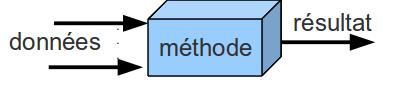
\includegraphics[width=0.8\linewidth,height=0.8\textheight,keepaspectratio=true]{/home/clr/Documents/Cours/DEV1Q2/TDModule/fr/image/methode.jpg}
						\end{center}
                
                    \caption[methode.jpg]{methode.jpg}
                \end{figure}
                    
            \par
         
		    Pour l'utiliser, il faut connaitre : 
		    
					\begin{itemize}
				
			\item son nom ;
			\item ce dont elle a besoin ;
			\item ce qu'elle retourne ;
			\item mais \textbf{pas comment} elle fait ;
					\end{itemize}
				
            \par
         
		    On peut appeler une m\'ethode 
		    
					\begin{itemize}
				
			\item \`a partir du code d'une autre classe : \,\verb|NomClasse.nomMéthode(...)|\,
			\item au sein de la m\^eme classe : \,\verb|nomMéthode(...)|\,
					\end{itemize}
				
            \par
        \subsection{Exemples}Par exemple : 
            \par
        \begin{Java}

public static double moyenne ( double nb1, double nb2 ) {
    double moyenne = (nb1 + nb2) / 2.0;
    return moyenne;
}				\end{Java}
        Appel possible (si dans la m\^eme classe) :
      
            \par
        \begin{Java}

double cote = moyenne(12.5, 17.5);
				\end{Java}Par exemple : 
            \par
        \begin{Java}

public static int absolu ( int nb ) {
    int abs;
    if (nb<0) {
      abs = -nb;
    } else {
      abs = nb;
    }
    return abs;
}				\end{Java}
        Appels possibles (si dans la m\^eme classe) :
      
            \par
        \begin{Java}

int resultat = absolu(4);
int ecart = -10;
int ecartAbsolu = absolu(ecart );
				\end{Java}Par exemple : 
            \par
        \begin{Java}

public static void presenter (String nomPgm) {
    System.out. println ("Programme "+nomPgm);
}				\end{Java}
        Appel possible (si dans la m\^eme classe) :
      
            \par
        \begin{Java}

presenter ("moyenne de 2 nombres");
				\end{Java}Par exemple : 
            \par
        \begin{Java}

public static int lireEntier () {
    Scanner clavier = new Scanner(System.in);
    int nb;
    System.out. println ("Entrez un nombre entier!");
    nb = clavier . nextInt ();
    return nb;
}				\end{Java}
        Appel possible (si dans la m\^eme classe) :
      
            \par
        \begin{Java}

int nb = lireEntier ();
				\end{Java}Montrons par un exemple comment \'ecrire la m\'ethode max2 : 
            \par
        \begin{Java}

import java.util.Scanner;
public class Test{
  public static double max2(double nb1, double nb2){
    double max = nb1;
		if (nb1 < nb2) {
			max = nb2;
		}
		return max;
  }
}				\end{Java}\subsection{Commenter une m\'ethode}
					\begin{itemize}
				
			\item 
            Pour qui ?
            
					\begin{itemize}
				
			\item Le programmeur qui va utiliser le code
			\item Le programmeur qui va maintenir le code (peut-\^etre vous)
					\end{itemize}
				
			\item 
              Quel type de documentation ?
            
					\begin{itemize}
				
			\item Ce que fait la m\'ethode/classe
			\item Comment elle le fait (peut \^etre r\'eduit au minimum si code lisible)
					\end{itemize}
				
			\item 
              Qui est int\'eress\'e par quoi ?
            
					\begin{itemize}
				
			\item Le programmeur-utilisateur : int\'eress\'e uniquement par le quoi
			\item Le programmeur-mainteneur : int\'eress\'e par le quoi et le comment
					\end{itemize}
				
			\item 
              O\`u mettre la documentation ?
            
					\begin{itemize}
				
			\item 
                Avec le code
                  
					\begin{itemize}
				
			\item Plus facile pour le maintenir
			\item Plus de chance de garder la synchronisation avec le code
					\end{itemize}
				
			\item Mais le programmeur-utilisateur n'a pas \`a voir le code pour l'utiliser
					\end{itemize}
				
					\end{itemize}
				
            \par
        
			
		\subparagraph{litterate programming} 
		
					\textcolor{white}{.} \par
				
					\begin{itemize}
				
			\item la documentation accompagne le code
			\item un outil extrait cette documentation pour en faire un document facile \`a lire
			\item toute la documentation suit la m\^eme structure, le m\^eme style -> plus facile \`a lire
					\end{itemize}
				
            \par
        
		    Regardons ce qui existe. 
		    Par exemple, la m\'ethode \verb@abs@ de la classe \verb@Math@ :
		  
            \par
        \begin{figure}[hbt]
				    \begin{center}
					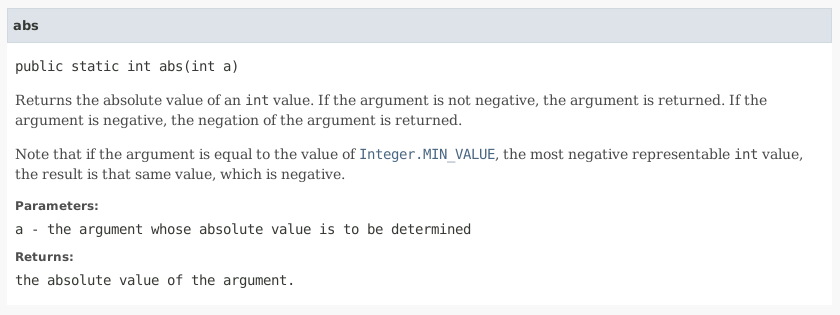
\includegraphics[width=0.8\linewidth,height=0.8\textheight,keepaspectratio=true]{/home/clr/Documents/Cours/DEV1Q2/TDModule/fr/image/Mathabs.png}
						\end{center}
                
                    \caption[Mathabs.png]{Mathabs.png}
                \end{figure}
                    
            \par
        
		    Il est essentiel de commenter chaque m\'ethode. C'est ce qui permet de pouvoir les utiliser facilement.
		  
            \par
        
		    Comment \'ecrire la n\^otre :
		  
            \par
        
			
		\subparagraph{javadoc} 
		
					\textcolor{white}{.} \par
				
					\begin{itemize}
				
			\item Le commentaire javadoc est identifi\'e par \verb@/**... */@ ;
			\item la documentation est produite au format HTML ;
			\item On commente essentiellement
            
					\begin{itemize}
				
			\item la classe : r\^ole et fonctionnement
			\item les m\'ethodes publiques : ce que \c ca fait, param\`etres et r\'esultats
					\end{itemize}
				
			\item Le commentaire se met \textbf{juste au dessus} de ce qui est comment\'e.
					\end{itemize}
				
            \par
        
			
		\subparagraph{Tag} 
		
					\textcolor{white}{.} \par
				
		    On utilise des \textbf{tags} pour identifier certains \'el\'ements.
		    Les plus courants :
		    
					\begin{itemize}
				
			\item @param : d\'ecrit les param\`etres
			\item @return : d\'ecrit ce qui est retourn\'e
			\item @throws : sp\'ecifie les exceptions lanc\'ees
			\item @author : note sur l'auteur
					\end{itemize}
				
            \par
        \begin{Java}

/**
* Donne la racine carree d un nombre.
* @param nb le nombre dont on veut la racine carree .
* @return la racine carree du nombre.
* @throws IllegalArgumentException si le nombre est negatif .
*/
public static double sqrt( double nb ) {
    if(nb<0) {
      throw new IllegalArgumentException("Nombre negatif");
    
    return Math.sqrt(nb);
}				\end{Java}
		    Exemple : la valeur absolue
      
            \par
        \begin{Java}

/**
* Calcul de la valeur absolue .
* @param nb le nombre dont on veut la valeur absolue .
* @return la valeur absolue de <code>nb</code>
*/
public static int absolu ( int nb ) {
    int abs;
    if (nb<0) {
      abs = -nb;
    } else {
      abs = nb;
    }
    return abs;
}				\end{Java}
					\begin{itemize}
				
			\item Les types sont d\'eduits de la signature et ajout\'es \`a la documentation.
			\item La premi\`ere phrase (termin\'ee par un \verb@.@) sert de r\'esum\'e.
					\end{itemize}
				
            \par
        
			
		\subparagraph{html} 
		
					\textcolor{white}{.} \par
				
		    La documentation peut contenir des balises HTML.
		  
            \par
        \begin{Java}

/**
* Indique si l annee est bissextile . Pour rappel :
* <ul>
*   <li>Une annee qui n est pas divisible par 4 n est pas bissextile (ex: 2009)</li>
*   <li>Une annee qui est divisible par 4</li>
*   <ul>
*     <li>est en general bissextile (ex: 2008)</li>
*     <li>sauf si c est un multiple de 100 mais pas de 400 (ex: 1900, 2100)</li>
*     <li>les multiples de 400 sont donc bien bissextiles (ex: 2000, 2400)</li>
*   </ul>
* </ul>
* Plus formellement, <code>a</code> est bissextile si et seulement si <br/>
* <code>a MOD 400 = 0 OU (a MOD 4 = 0 ET a MOD 100 != 0)</code>
* @param annee l annee dont on se demande si elle est bissextile
* @return vrai si l annee est bissextile
*/}				\end{Java}
        Ce qui donne : 
        \begin{figure}[hbt]
				    \begin{center}
					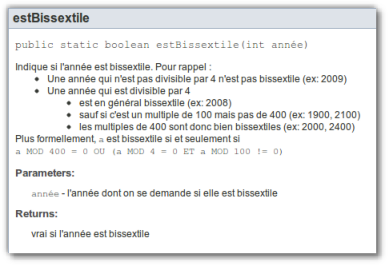
\includegraphics[width=0.8\linewidth,height=0.8\textheight,keepaspectratio=true]{/home/clr/Documents/Cours/DEV1Q2/TDModule/fr/image/javadocBissextile.png}
						\end{center}
                
                    \caption[javadocBissextile.png]{javadocBissextile.png}
                \end{figure}
                    
            \par
        
			
		\subparagraph{Produire la documentation} 
		
					\textcolor{white}{.} \par
				
        La commande javadoc : 
        
					\begin{itemize}
				
			\item javadoc Temps.java
			\item javadoc ∗.java
			\item javadoc −d doc ∗.java
			\item javadoc −charset utf−8 ∗.java
			\item . . . et beaucoup d'autres options (cf. documentation de javadoc)
					\end{itemize}
				
            \par
        
			
		\subparagraph{Une bonne documentation} 
		
					\textcolor{white}{.} \par
				
        Une bonne javadoc d\'ecrit le quoi mais jamais le comment -> ne jamais parler de ce qui est priv\'e.
      
            \par
        
        Mauvais exemples :
        
					\begin{itemize}
				
			\item On utilise un for pour parcourir le tableau.
			\item Pour aller plus vite, on stocke le \verb@prix hors tva@ dans une variable temporaire.
					\end{itemize}
				
            \par
        
        Ne pas \'ecrire ce que javadoc \'ecrit lui-m\^eme :
      
            \par
        
        Mauvais exemples :
        
					\begin{itemize}
				
			\item nb - un entier qui ...
			\item La m\'ethode sqrt ...
			\item Cette m\'ethode ne retourne rien.
					\end{itemize}
				
            \par
        
        Pour en savoir plus : 
        http://www.oracle.com/technetwork/articles/java/index-137868.html (\url{www.oracle.com/technetwork/articles/java/index-137868.html})
            \par
        \subsection{Un exemple complet}\begin{Java}

import java. util .Scanner;
public class MaxEntiers {
    /**
    * Donne le maximum de 2 nombres.
    * @param nb1 le premier nombre.
    * @param nb2 le deuxieme nombre.
    * @return la valeur la plus grande entre <code>nb1</code> et <code>nb2</code>
    */
    public static int max ( int nb1, int nb2 ) {
      int max=0;
      if (nb1 > nb2) {
        max = nb1;
      } else {
        max = nb2;
      }
      return max;
    }
    
    /**
    * Lit un nombre entier .
    * Le nombre est lu sur l entree standard ( le clavier ).
    * @return le nombre entier lu .
    */
    public static int lireEntier () {
    Scanner clavier = new Scanner(System.in);
    System.out. println ("Entrez un nombre entier!");
      return clavier . nextInt ();
    }
    
    /**
    * Affiche le maximum de 2 nombres entres au clavier.
    * @param args pas utilise.
    */
    public static void main ( String [] args ) {
      int max; // Le max des nombres lus
      int nb1, nb2; // Chacun des nombres lus
      nb1 = lireEntier ();
      nb2 = lireEntier ();
      max = max(nb1,nb2);
      System.out. println ("max = " + max);
    }
}				\end{Java}\section{Exercices}
				Maintenant, mettons tout \c ca en pratique.
      
            \par
        \subsection{Compr\'ehension d'algorithme}
          Pour ces exercices, nous vous demandons de comprendre des algorithmes donn\'es. 
          
			
		\subparagraph{Compr\'ehension} 
		
                \textcolor{white}{.} \par
            
							  Que vont-ils afficher ?
              
					\begin{itemize}
				
			\item \begin{verbatim}
module ex1 ()
    x, y : entiers
    addition(3, 4, x)
    afficher x
    x ← 3
    y ← 5
    addition(x, y, y)
    afficher y
fin module

module addition(a↓, b↓, c↑ : entiers)
    somme : entier
    somme ← a + b
    c ← somme
fin module
				\end{verbatim} \textcolor{gray}{\underline{\hspace*{1em}}}  \textcolor{gray}{\underline{\hspace*{1em}}} 
			\item \begin{verbatim}
module ex2 ()
    a, b : entiers
    addition(3, 4, a)
    afficher a
    a ← 3
    b ← 5
    addition(b, a, b)
    afficher b
fin module

module addition(a↓, b↓, c↑ : entiers)
    somme : entier
    somme ← a + b
    c ← somme
fin module
				\end{verbatim} \textcolor{gray}{\underline{\hspace*{1em}}}  \textcolor{gray}{\underline{\hspace*{1em}}} 
			\item \begin{verbatim}
module ex3 ()
    a, b, c : entiers
    calcul(3, 4, c)
    afficher c
    a ← 3
    b ← 4
    c ← 5
    calcul(b, c, a)
    afficher a, b, c
fin module

module calcul(a↓, b↓, c↑ : entiers)
    a ← 2*a
    b ← 3*b
    c ← a+b
fin module
				            \end{verbatim} \textcolor{gray}{\underline{\hspace*{2em}}}  \textcolor{gray}{\underline{\hspace*{2em}}} 
			\item \begin{verbatim}
module ex4 ()
    a, b, c : entiers
    a ← 3
    b ← 4
    c ← f(b)
    afficher c
    calcul2(a, b, c)
    afficher a, b, c
fin module

module calcul2 (a↓, b↓, c↑ : entiers)
    a ← f(a) 
    c ← 3*b 
    c ← a+c
fin module

module f (a↓ : entier) → entier
    b : entier
    b ← 2*a+1
    retourner b
fin module
				            \end{verbatim} \textcolor{gray}{\underline{\hspace*{1em}}}  \textcolor{gray}{\underline{\hspace*{1em}}}  \textcolor{gray}{\underline{\hspace*{1em}}}  \textcolor{gray}{\underline{\hspace*{2em}}} 
					\end{itemize}
				
            \par
        \subsection{Compr\'ehension de codes Java}
          Pour ces exercices, nous vous demandons de comprendre des codes Java donn\'es. 
          
			
		\subparagraph{Compr\'ehension} 
		
                \textcolor{white}{.} \par
            
							  ***********************************A FAIRE***************************************************
							  Que vont-ils afficher si \`a chaque fois les deux nombres lus au d\'epart sont successivement 2, 3 et 4 ?
							
					\begin{itemize}
				
			\item \begin{Java}
import java.util.Scanner;
public class Exercice1 {
    public static void main(String [] args) {
        Scanner clavier = new Scanner(System.in);
        int nb1 = clavier.nextInt();
        int nb2 = clavier.nextInt();
        int nb3 = clavier.nextInt();
        if (nb1 < nb2){
          System.out.println(nb1);
        } else {
          System.out.println(nb2);
        } 
    }
}
        \end{Java} \textcolor{gray}{\underline{\hspace*{1em}}} 
			\item \begin{Java}
import java.util.Scanner;
public class Exercice2 {
    public static void main(String [] args) {
        Scanner clavier = new Scanner(System.in);
        int nb1 = clavier.nextInt();
        int nb2 = clavier.nextInt();
        int nb3 = clavier.nextInt();
        if (nb1 > nb2 && nb1 > nb3){
          System.out.println(nb1);
        } else {
            if (nb2 > nb3){
              System.out.println(nb2);
            } else {
              System.out.println(nb3);
            }
        } 
    }
}
        \end{Java} \textcolor{gray}{\underline{\hspace*{1em}}} 
			\item \begin{Java}
import java.util.Scanner;
public class Exercice3 {
    public static void main(String [] args) {
        Scanner clavier = new Scanner(System.in);
        int nb1 = clavier.nextInt();
        int nb2 = clavier.nextInt();
        int nb3 = clavier.nextInt();
        switch (nb1){
          case 1 : System.out.println("premier"); break;
          case 2 : System.out.println("deuxieme"); break;
          case 3 : System.out.println("troisieme"); break;
          default : System.out.println("pas dans le trio");
        } 
    }
}
        \end{Java} \textcolor{gray}{\underline{\hspace*{10em}}} 
			\item \begin{Java}
import java.util.Scanner;
public class Exercice3 {
    public static void main(String [] args) {
        Scanner clavier = new Scanner(System.in);
        int nb1 = clavier.nextInt();
        int nb2 = clavier.nextInt();
        int nb3 = clavier.nextInt();
        switch (nb1){
          case 1 : System.out.println("premier");
          case 2 : System.out.println("deuxieme");
          case 3 : System.out.println("troisieme");
          default : System.out.println("pas dans le trio");
        } 
    }
}
        \end{Java} \textcolor{gray}{\underline{\hspace*{20em}}} 
					\end{itemize}
				
            \par
        \subsection{\`A vous de jouer...}
          Il est temps de se lancer et d'\'ecrire vos premiers modules et programmes Java correspondant. 
          Voici quelques conseils pour vous guider dans la r\'esolution de tels probl\`emes :
          
					\begin{itemize}
				
			\item il convient d'abord de bien comprendre le probl\`eme pos\'e ; assurez-vous qu'il est parfaitement sp\'ecifi\'e ;
			\item d\'eclarez ensuite les variables (et leur type) qui interviennent dans l'algorithme ; les noms des variables risquant de ne pas \^etre suffisamment explicites ;
			\item mettez en \'evidence les variables \guillemotleft  donn\'ees \guillemotright , les variables \guillemotleft  r\'esultats \guillemotright  et les variables de travail ;
			\item n'h\'esitez pas \`a faire une \'ebauche de r\'esolution en fran\c cais avant d'\'elaborer l'algorithme d\'efinitif pseudo-cod\'e.
			\item \'Ecrivez la partie algorithmique \textbf{AVANT} de vous lancer dans la programmation en Java.
					\end{itemize}
				
            \par
        
        \'Ecrivez les algorithmes et codez les programmes Java correspondant qui 
          
					\begin{enumerate}
				
			\item \'echange le contenu de deux variables enti\`eres pass\'ees en param\`etres.
            
			\item retourne le maximum de 4 nombres donn\'es en param\`etre en utilisant 
              les modules \verb@max2@ et/ou \verb@max3@ d\'ej\`a d\'evelopp\'es dans ce chapitre.
			\item valide une date donn\'ee par trois entiers : l'ann\'ee, le mois et le jour.
			\item \'etant donn\'e trois nombres, recherche et affiche si le premier des 
            trois appartient \`a l'intervalle donn\'e par le plus petit et le plus grand des deux autres (bornes exclues). 
            Qu'est-ce qui change si on inclut les bornes ?
			\item \'etant donn\'e une \'equation du deuxi\`eme degr\'e, d\'etermin\'ee par le coefficient de x\texttwosuperior  , le coefficient de x et le terme ind\'ependant, 
            recherche et affiche la (ou les) racine(s) de l'\'equation (ou un message ad\'equat s'il n'existe pas de racine r\'eelle).
			\item \`a partir d'un moment exprim\'e par 2 entiers, heure et minute, affiche le moment qu'il sera une minute plus tard.
			\item v\'erifie si une ann\'ee est bissextile. Pour rappel, les ann\'ees bissextiles sont les ann\'ees multiples de 4.
             Font exception, les multiples de 100 (sauf les multiples de 400 qui sont bien bissextiles). Ainsi 2012 et 2400 sont bissextile mais pas 2010 ni 2100.
			\item Dans une rue o\`u se pratique le stationnement alternatif, du 1 au 15 du mois, on se gare du c\^ot\'e des maisons ayant un num\'ero impair, 
            et le reste du mois, on se gare de l'autre c\^ot\'e.
            \'Ecrivez un algorithme et le code java correspondant qui, sur base de la date du jour et du num\'ero de maison devant laquelle
            vous vous \^etes arr\^et\'e, indique si vous \^etes bien stationn\'e ou non.
					\end{enumerate}
				
            \par
        
				\end{document}
			